\documentclass[oneside, astronomy, noacknowlegments]{BYUPhys}

% Your name
  \Author{Scott Leland Crossen}

% Enter the date your thesis is approved
  \Year{[Year]}
  \Month{[Approval Month]}

% If you have a long title, split it between multiple lines using the \\ command
  \Title{Optically Detected Magnetic Resonance;
Computational Predictions\\and Experimental Results
  }

% Your research advisor
\AdvisorTitle{Advisor}
  \Advisor{Dr. John S. Colton}

% For honors theses, enter the name of the honors Representative
  \HonorsRepresentative{Kristine Hansen}

% The text of your abstract
  \Abstract{ [The abstract is a summary of the thesis/dissertation
  with emphasis on the findings of the study. The abstract must not
  exceed 350 words in length and fit on one page, single spaced.] }

 \Keywords{[A comma-separated list of descriptive words for search purposes]}

% Acknowledge those who helped and supported you
  \Acknowledgments{
    [Acknowledgements should be simple, in good taste, and fit on one page]
  }

%% The members of your committee (masters only need A and B, PhD need all 4)
%  \MemberA{Committee Member A}
%  \MemberB{Committee Member B}
%  \MemberC{Committee Member C}
%  \MemberD{Committee Member D}
%

\begin{document}

 % Start page counting in roman numerals
 \frontmatter

 % This command makes the formal preliminary pages.
 % You can comment it out during the drafting process if you want to save paper.
 \makepreliminarypages

 % Make the table of contents.
 \tableofcontents

 % Start regular page counting at page 1
 \mainmatter

% OK. Everything is set up. Type your thesis here.
\listoffigures 


\chapter{Introduction}

\section{Qualitative Description of ESR and ODMR}
\label{sec:Qualitative}

\textit{Optically Detected Magnetic Resonance} (ODMR) is a particular form of \textit{Electron Paramagnetic Resonance} (EPR) which is more commonly known as \textit{Electron Spin Resonance} (ESR). The latter two of these terms (EPR and ESR) are synonymous; The former (ODMR) is a particular subset of ESR that utilizes a luminescence measuring technique as a means to collect ESR information. In literature, it is common to see both of these terms followed by the designation "spectroscopy" - as that is what they are: tools to study properties of matter via electromagnetic radiation. Though the extent of their application has grown over the years, ESR and ODMR are most commonly used to study the spin-properties of electrons and electron-holes trapped in metal lattices. They can be used to study free radicals in organic materials and are also important in studying the local environment of lattice defects through a technique using angular-dependent ODMR. One particular use of ODMR is the study of electron-spin coherence via a technique known as \textit{Electron Spin Echo}. This can be useful when studying what properties and conditions lead to superior state coherence for qubit candidate materials in quantum computing.

The intellectual foundation of Electron Spin Resonance is rooted in Quantum Mechanics. Bound electrons in matter have discrete and quantized energy levels that govern what frequencies of light are emitted when transitions between energy levels are made. For electron systems, which are fermions and thus subject to the Pauli exclusion principle, the energy levels are 2nd order degenerate when bound in matter. In Quantum Mechanics we choose to describe this degeneracy in terms of spins: we say an electron is either "spin-up" or "spin-down". Each energy level can have at most two electrons of opposite spins inhabiting it (and thus the degeneracy). The spin terminology is arbitrary however, and is really just an attempt at comparing electrons to particles. In truth, electron spin is a meaningless term for a property that is emergent from solving the wave function but it nonetheless describes a principle of conservation of momentum that would be found in classical system such as a top and so the term makes sense and has persisted. In this case the electron’s spin is a description of the magnetic moment when the particle is in the presence of a magnetic field. In the case of electrons bound in matter, the energy levels of the molecule will split according to the "Zeeman Effect" and the spin-states of the electrons can be observed - most commonly through a photoluminescence or other fluorescence measuring technique.

The Zeeman effect itself is crucial in understanding the principles of ESR. In the presence of a magnetic field, populations of free electrons will form a spin-1/2 system between a higher-energy "spin-up" state and a lower-energy "spin-down" state. In matter, different parities of spin-states can be formed between the interactions of different energy levels with different transition selection-rules. A spin-1/2 system in the presence of a magnetic field is shown in \ref{fig:Zeeman}. As seen, the energy levels of the two differing spins diverge linearly for an increasing magnetic field. The difference in energy between these two levels is typically in the microwave frequency domain. For a given magnetic-field strength there will be a set of characteristic microwave frequencies that the electrons are most likely at emitting when transitioning between these quantized states. In a spin-1/2 system there will only be one frequency for a given magnetic field corresponding to the difference between the two zeeman lines at that given field strength. Likewise, for a given microwave target signal, there will be a variety of magnetic field strengths which are most adept at transitioning bound electrons between states. This unique pairing between both the microwave frequency and magnetic field strength is the resonant condition that ESR is based off of and also the means that it uses to discover information about materials.

\begin{figure}
    \caption[Zeeman effect and resonant conditions in matter]{\label{fig:Zeeman}
     This is the figure description.}
\end{figure}

\section{The Defect Nature of Materials}
\label{sec:Defects}

\section{Electron Spin, Quantum Computing, and Qubits}
\label{sec:QuantumComputers}

Classical Computation is almost always based off of a binary system. In these architectures, the computer’s register, memory, and general logical states are either in a logical ‘true’ or a logical ‘false’ state. A ‘true’ state corresponds to a high voltage and a ‘false’ state corresponds to a grounded voltage. A computer’s bits can be in either of these two states - 1 or 0 - but not both.

A spin-1/2 system also describes a binary system between a higher-energy basis state and a lower-energy basis state. In this comparison, the spin-1/2 system will be measured (and the wave function collapsed) to be in either of these two states - but not both. The important difference between the the spin-1/2 system and the classical bit model is that the spin system can have states that exist as linear combinations of the two basis up/down states. In accordance with Quantum Mechanics, this means that the spin-1/2 system can exist as a superposition between both the spin-up and spin-down states and has a certain probability of being measured in each. It is important to note that the superposition mentioned does not mean that the state exists as some value in between an excited state and a lower state. Rather, it exists as both states simultaneously.

Because of this unique property of spin systems, they can then be used as the basis for forming what is called a “quantum computer”. Though it depends on the architecture, Quantum computers can be thought of to manipulate information in a similar fashion to that of a quantum computer. Both have logical operators and storage bits and both are algorithmically based. Quantum computers, however, utilize this unique possibility of superposition to make probabilistic calculations for many different states at once. This happens through the quantum mechanical operators that initialize and manipulate the states which are stored in “qubits” - or the quantum computer version of classical bits that can exist in these types of states. Because of the existing construction from nondeterministic finite automata to deterministic finite automata, quantum computers are also turing complete in the broad definition of that term.

Today, there is large emphasis within the scientific community in building viable, scalable quantum computers. The reason for this is that quantum computers offer reduced computational times for certain types of algorithms. Certainly however, these machines are not necessarily more adept at processing videos to be scrubbed by common users, but are rather designed to carry out a few types of intense calculations in logarithmic time that would normally have a polynomial time dependence. The most notable use for quantum computers in our modern society is within the field of computer security and encryption. Quantum computers have the ability to compute prime factors via Shor’s algorithm in a much faster time than traditional computers. This ability would essentially render all of the current RSA encryption methods obsolete in addition to anything that relies on public/private key encryption such as bitcoin.

Although more than just spin systems can be used as the all-important qubits for quantum computing, we will focus on this type - specifically spin-1/2 systems formed from electrons - for the basis of our discussion. As mentioned earlier, Electron Spin Resonance is the major tool used to study the spin properties of materials. In the case of quantum computation, ESR is used to study possible qubit materials that might eventually be used in such machines. Currently, one of the major difficulties in creating quantum computers is to find materials that can form superposition states that remain coherent (and reliable) over prolonged periods of time. In order to understand what properties of materials lead to superior qubit construction and state coherence, ESR can be used in conjunction with electron spin echo experiments to study the coherence of electrons in a spin-1/2 system. Moreover, ESR can be used alone to study the spin system itself and the local environment of the defects in matter that form them. Knowledge of this important topic will serve to increase our ability to construct better qubits for use in quantum computers.

\section{}
\section{}

\begin{figure}
    \centerline{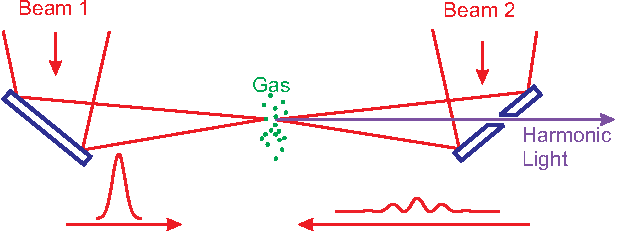
\includegraphics{Graphic1}}
    \caption[Magnetic field and microwave frequency relationship]{\label{fig:MFRelationship}
     A mirror with a hole is used to extract high-order harmonics generated in
     counter-propagating laser beams.}
 \end{figure}

\section{}
\section{}

\chapter{Computational Model and Theory}
\section{}
\section{}
\section{Spin Hamiltonians and Defect-State Contributions}

\begin{figure}
    \centerline{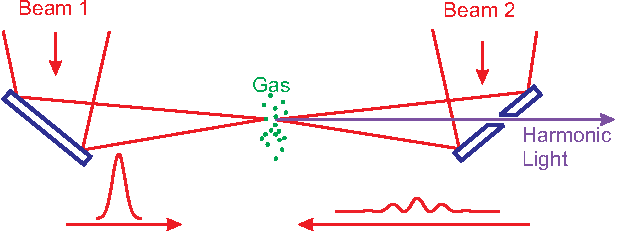
\includegraphics{Graphic1}}
    \caption[Example of spin-hamiltonion fields]{\label{fig:HamFields}
     A mirror with a hole is used to extract high-order harmonics generated in
     counter-propagating laser beams.}
 \end{figure}

\section{}
\section{}

\chapter{Experimental Methods}
\section{}
\section{}
\section{Experiment Background}

\begin{figure}
    \centerline{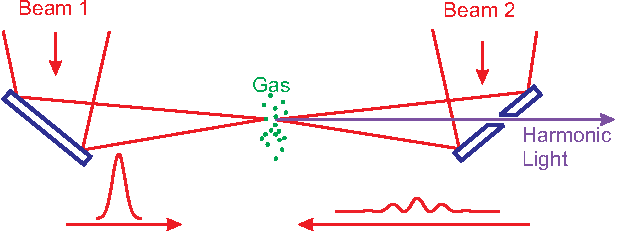
\includegraphics{Graphic1}}
    \caption[SiC energy levels and zero-field splitting]{\label{fig:SiCZeeman}
     A mirror with a hole is used to extract high-order harmonics generated in
     counter-propagating laser beams.}
 \end{figure}

\section{}

\chapter{Results}
\section{Computational Predictions}

\begin{figure}
    \centerline{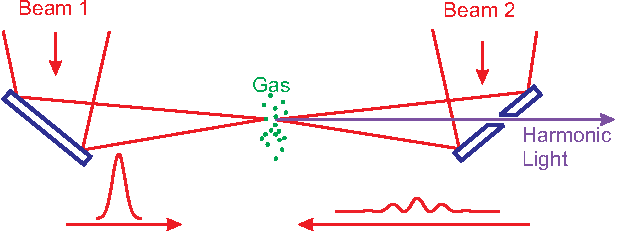
\includegraphics{Graphic1}}
    \caption[ODMR computational model for SiC]{\label{fig:SiCModel}
     A mirror with a hole is used to extract high-order harmonics generated in
     counter-propagating laser beams.}
 \end{figure}

\begin{figure}
    \centerline{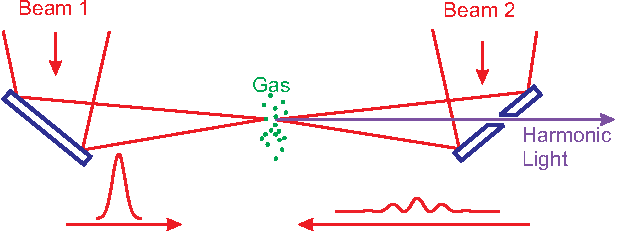
\includegraphics{Graphic1}}
    \caption[ODMR computational model for CdTe]{\label{fig:CdTeModel}
     A mirror with a hole is used to extract high-order harmonics generated in
     counter-propagating laser beams.}
 \end{figure}

\section{Experimental Results}

\begin{figure}
    \centerline{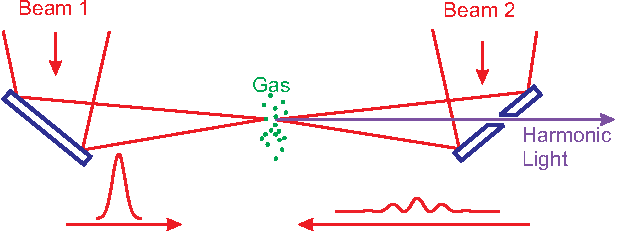
\includegraphics{Graphic1}}
    \caption[Experimental ODMR for SiC]{\label{fig:SiCResults}
     A mirror with a hole is used to extract high-order harmonics generated in
     counter-propagating laser beams.}
 \end{figure}

\begin{figure}
    \centerline{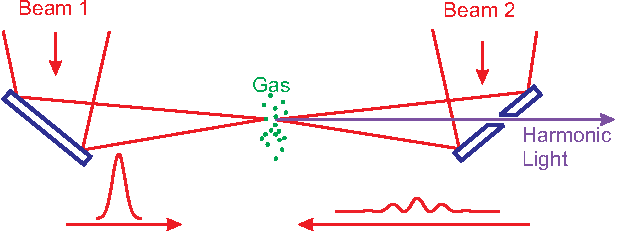
\includegraphics{Graphic1}}
    \caption[Experimental ODMR for CdTe]{\label{fig:CdTeResults}
     A mirror with a hole is used to extract high-order harmonics generated in
     counter-propagating laser beams.}
 \end{figure}


\section{}
\section{}


\begin{appendices}

\chapter{Electron Spin Studies of Electron Irradiated SiC}
\label{sec:appenda}

\begin{figure}
    \centerline{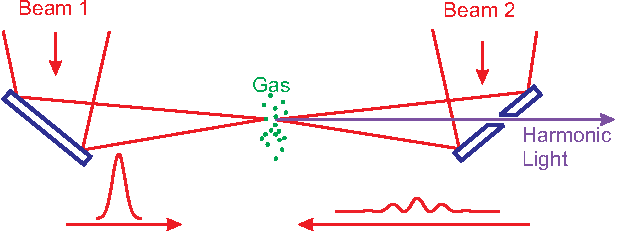
\includegraphics{Graphic1}}
    \caption[Electron-irradiated SiC lifetime  summary]{\label{fig:e17results}
     A mirror with a hole is used to extract high-order harmonics generated in
     counter-propagating laser beams.}
 \end{figure}

\begin{figure}
    \centerline{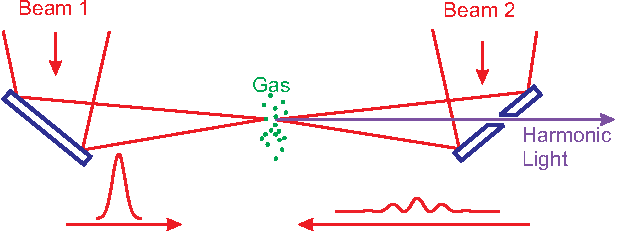
\includegraphics{Graphic1}}
    \caption[ODMR/Photoluminescence vs temperature]{\label{fig:ODMRPL}
     A mirror with a hole is used to extract high-order harmonics generated in
     counter-propagating laser beams.}
 \end{figure}

\chapter{Optical Studies of Cadmium Telluride}
\label{sec:appendb}


word
\cite{RefWorks:doc:58929816e4b0499fa95c51a6}
\cite{RefWorks:doc:58929629e4b0d4c09201f6b8}
\cite{RefWorks:doc:589299f4e4b0d4c09201f915}
\cite{RefWorks:doc:58929128e4b0228a292928a7}
\cite{RefWorks:doc:589299fbe4b0dec22aee3bd8}
\cite{RefWorks:doc:5892912ae4b0dec22aee3993}
\cite{RefWorks:doc:58929128e4b0499fa95c5064}
\cite{RefWorks:doc:5892989ee4b0499fa95c51c8}
\cite{RefWorks:doc:589293f5e4b0dec22aee39de}
\cite{RefWorks:doc:589295fce4b0d4c09201f6b4}
\cite{RefWorks:doc:58929a02e4b0d4c09201f91b}
\cite{RefWorks:doc:589295bde4b0d4c09201f692}
\cite{RefWorks:doc:58929264e4b0d4c09201f63b}
\cite{RefWorks:doc:58929129e4b0d4c09201f61e}
\cite{RefWorks:doc:58929602e4b0d4c09201f6b6}
\cite{RefWorks:doc:589296c6e4b0d4c09201f6f5}
\cite{RefWorks:doc:58929746e4b0dec22aee3a9a}
\cite{RefWorks:doc:589297a9e4b0d4c09201f736}
\cite{RefWorks:doc:58929800e4b0499fa95c51a1}
\cite{RefWorks:doc:589299f0e4b0dec22aee3bd6}
\cite{RefWorks:doc:58929786e4b0228a292929b8}
\cite{RefWorks:doc:58929612e4b0499fa95c50fa}
\cite{RefWorks:doc:5892964ee4b0499fa95c5108}
\cite{RefWorks:doc:58929c15e4b0228a29292c58}
\cite{RefWorks:doc:5892912ae4b0228a292928aa}




\begin{figure}
    \centerline{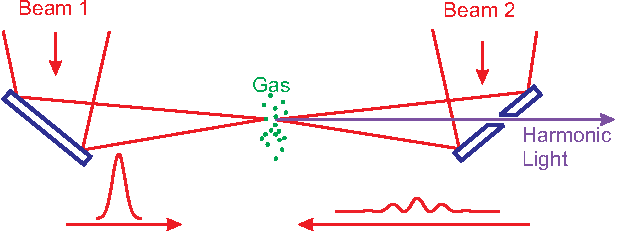
\includegraphics{Graphic1}}
    \caption[Photoluminescence of CdTe]{\label{fig:CdTePL}
     A mirror with a hole is used to extract high-order harmonics generated in
     counter-propagating laser beams.}
 \end{figure}

\chapter{Electron Spin Coherence of Silicon Vacancies in Proton-Irradiated 4H-SiC}
\label{sec:appendc}

\end{appendices}



%\chapter{A Sample Chapter}
%
%\section{A Fascinating Section}
%\label{sec:meaningfulname}
%
%For a short thesis, you can usually just type the whole body of the
%thesis here.  For longer documents you might consider typing
%chapters in separate files and using the \verb|\include| command.
%There is another example on the physics web page
%(\href{http://www.physics.byu.edu/undergraduate/latex.aspx}{click
%here to go there}) that shows how to do this.
%
%You can create your bibliography right in the main tex document.
%Here are references to a book \cite{Jackson1998}, an article
%\cite{Peatross2000}, and a web site \cite{intel}. You can also use
%BibTeX to keep track of your references.  The method for using
%BibTeX is shown in the other example on the physics web page.
%
%Making an index is easy. Just use the \verb|\index{Key}| command.
%\index{Index!Making} You can include figures too (see
%Fig.~\ref{fig:MirrorDiagram}).  Usually you need both eps and pdf
%versions of each figure.
%\begin{figure}
%    \centerline{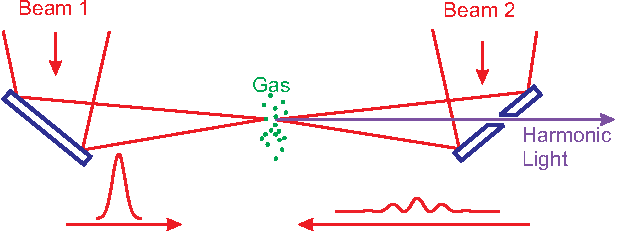
\includegraphics{Graphic1}}
%    \caption[Setup for using counter-propagating light]{\label{fig:MirrorDiagram}
%     A mirror with a hole is used to extract high-order harmonics generated in
%     counter-propagating laser beams.}
% \end{figure}







% Make the bibliography.
% Enter your references in the BibTex file "references.bib"
 \bibliography{references}

% Make the index
 \printindex

\end{document}
